\section{Cơ sở thiết kế trò chơi}
\subsection{Tổng quan trò chơi}
\hspace*{0.5cm} \textbf{MeowSQL Knight} là một trò chơi nhập vai Phiêu lưu chiến đấu theo lượt. Thay vì sử dụng các thao tác thông thường bằng các nút, người chơi tương tác bằng các nhập câu truy vấn và thực thi chúng, thu thập dữ kiện để chiếm lấy ưu thế trong chiến đấu, đánh bại quái vật và hoàn thành màn chơi.\\
\begin{figure}[H]
	\centering
	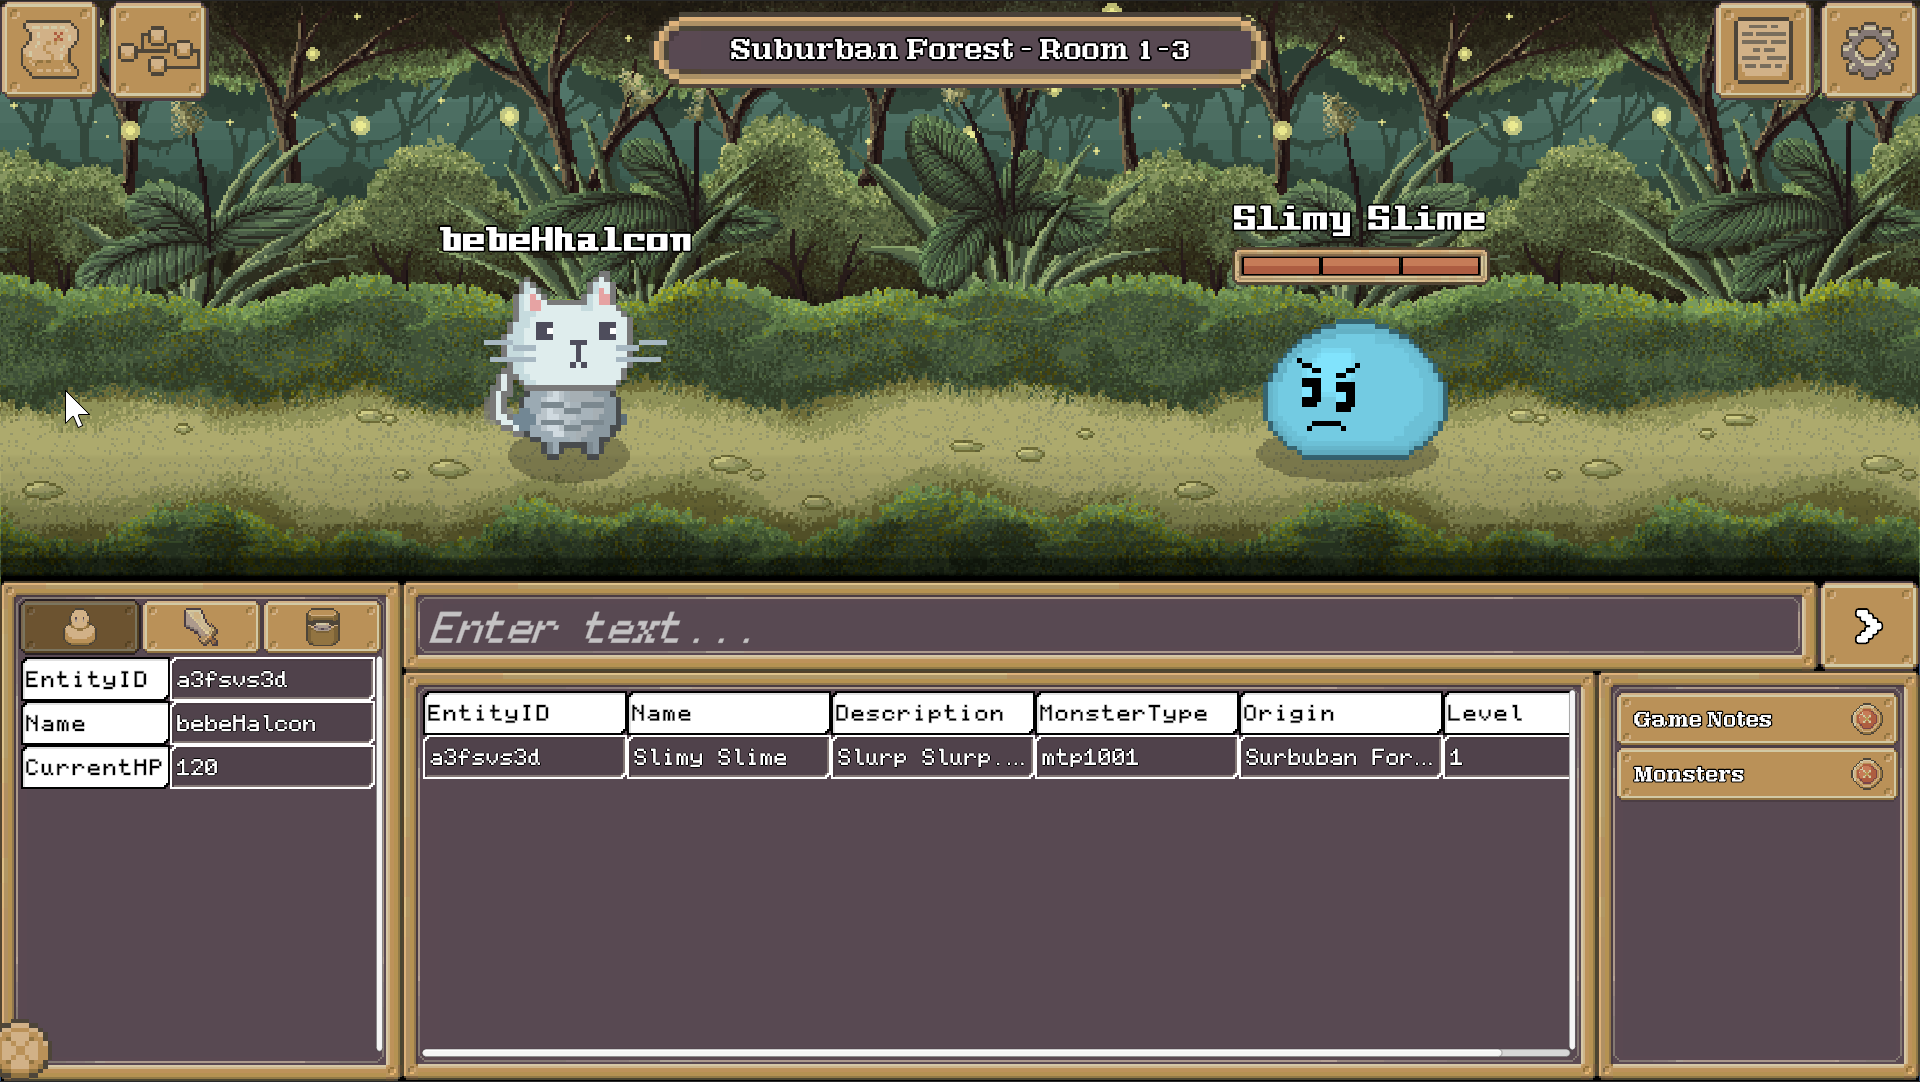
\includegraphics[width=\textwidth]{Images/Overall.png}
	\vspace{0.5cm}
	\caption{Tổng quan một màn chơi trong MeowSQL Knight}
\end{figure}
\hspace*{0.5cm} Người chơi sẽ sử dụng các câu truy vấn để khai thác cơ sở dữ liệu có cấu trúc cho sẵn. Sử dụng \textbf{select} để truy xuất dữ liệu của bảng và hiện kết quả lên màn hình, thu thập thông tin từ những dữ liệu đã hiện đó. Ngoài ra cũng có thể \textbf{insert}, \textbf{update} và \textbf{delete} những record trên bảng đặc biệt mang chức năng thực hiện hành động hoặc những bảng được phép, trò chơi sẽ phản ứng với hành động của người chơi như thế nào. Người chơi sẽ tấn công quái vật bằng các vũ khí mà người chơi mang vào trận chiến, cũng như sử dụng các kỹ năng. Để tương tác với game (tấn công quái vật, dùng vật phẩm), người chơi sẽ insert các tham số vào các bảng có chức năng đặc biệt, sau khi chèn xong thì hành động sẽ được thực thi.\\
\hspace*{0.5cm} Trong Schema này, các thực thể như người chơi, quái vật, bộ phận chí mạng của quái vật,... đều thuộc chung một bảng và có chung mã định danh như nhau. Để tiêu diệt quái vật, người chơi phải xác định được ID của chúng để có thể tấn công chính xác, bằng không các đòn đánh của người chơi sẽ bị trượt.\\
\hspace*{0.5cm} Người chơi phải tìm cách khai thác schema một cách hiệu quả trong chiến đấu. Đi kèm với việc lựa chọn trang bị hợp lý để giành chiến thắng, hoàn thành màn chơi và đi sâu hơn để tìm ra bí ẩn của trò chơi.


\subsection{Sơ lược cốt truyện}
\hspace*{0.5cm} Trong một thế giới game RPG có chủ đề là động vật bình thường, bạn là một kỵ sĩ mèo đang đi rừng để tìm nguyên liệu, mọi thứ diễn ra một cách bình thường. \\
\hspace*{0.5cm} Đột nhiên, trò chơi bỗng hoạt động không đúng so với trước kia, các quái vật trở nên hung hãn hơn, nguy hiểm hơn, lẽ ra chỉ cần đánh bằng các phương pháp thông thường đã có thể diệt sạch chúng, nhưng kì lạ thay, các phương pháp thông thường không còn có hiệu quả với chúng nữa. Đám quái vật vùng lên làm loạn cả thế giới game, khiến thế giới game bị lỗi nghiêm trọng, và nếu cứ tiếp tục như vậy, trò chơi sẽ không thể chơi được nữa.\\
\hspace*{0.5cm} Chính lúc này, nhân vật chính của chúng ta bị một con slime bao vây, lẽ ra 1 nhát từ kiếm của cậu có thể hạ gục con Slime, tuy nhiên, trong thế giới game bị rối loạn như thế này là không thể. Cậu cứ đánh trong vô vọng, trong khi con quái vật giận dữ tiến gần định nuốt chửng cậu. Đột nhiên, một tia sáng xuất hiện giết chết con quái vật đó. Là Nhà phát triển (Dev) của trò chơi này. Anh ấy đã kiểm tra hệ thống thế giới game và phát hiện ra bạn là một trong những object hiếm hoi còn sống trong thế giới game này. Để hỗ trợ bạn, Dev cấp cho bạn 1 năng lực lớn: bạn có thể xem schema của game và thực hiện các câu truy vấn SQL để khai thác schema và chiến đấu. Vì chỉ có sử dụng SQL mới có thể đánh bại các quái vật SQL. \\
\hspace*{0.5cm} Dev muốn đặt niềm tin vào bạn vì Dev không thể khởi dộng lại Project game này, nó là một project chạy trên server nhưng cậu đã mất quyền kiểm soát cả server và project. Dev muốn bạn đi sâu vào bên trong lõi của game và tìm ra lý do khiến game trở nên như vậy. Bạn là hy vọng của thế giới game này, và là hy vọng của cả Dev. Bạn bắt đầu đi vào sâu trong thế giới, mang sứ mệnh vô cùng cao cả, không chỉ để cứu thế giới này.

\subsection{So Sánh các sản phẩm tương tự trên thị trường}
\hspace*{0.5cm} Nhắc đến dòng game giải đố theo lượt chúng ta không thể bỏ qua series game \textbf{Bookworm Adventures} được phát triển bởi \textit{\textbf{PopCap Games}}. Đây là một trong những trò chơi độc đáo kết hợp giữa ghép chữ và chiến đấu theo lượt, tạo ra phong cách riêng biệt và mới mẻ trong dòng game này.\\
\hspace*{0.5cm} Ở thời điểm hiện tại, trò chơi giải đố dựa trên cấu trúc của ngôn ngữ lập trình SQL đã xuất hiện trong một số sản phẩm. Sản phẩm nổi bật nhất là \textbf{SQL Murder Mystery} được phát triển bởi \textit{\textbf{Knight Lab}} của Đại học Northwestern, Mỹ.
\begin{figure}[H]
\centering
\begin{minipage}{.5\textwidth}
  \centering
  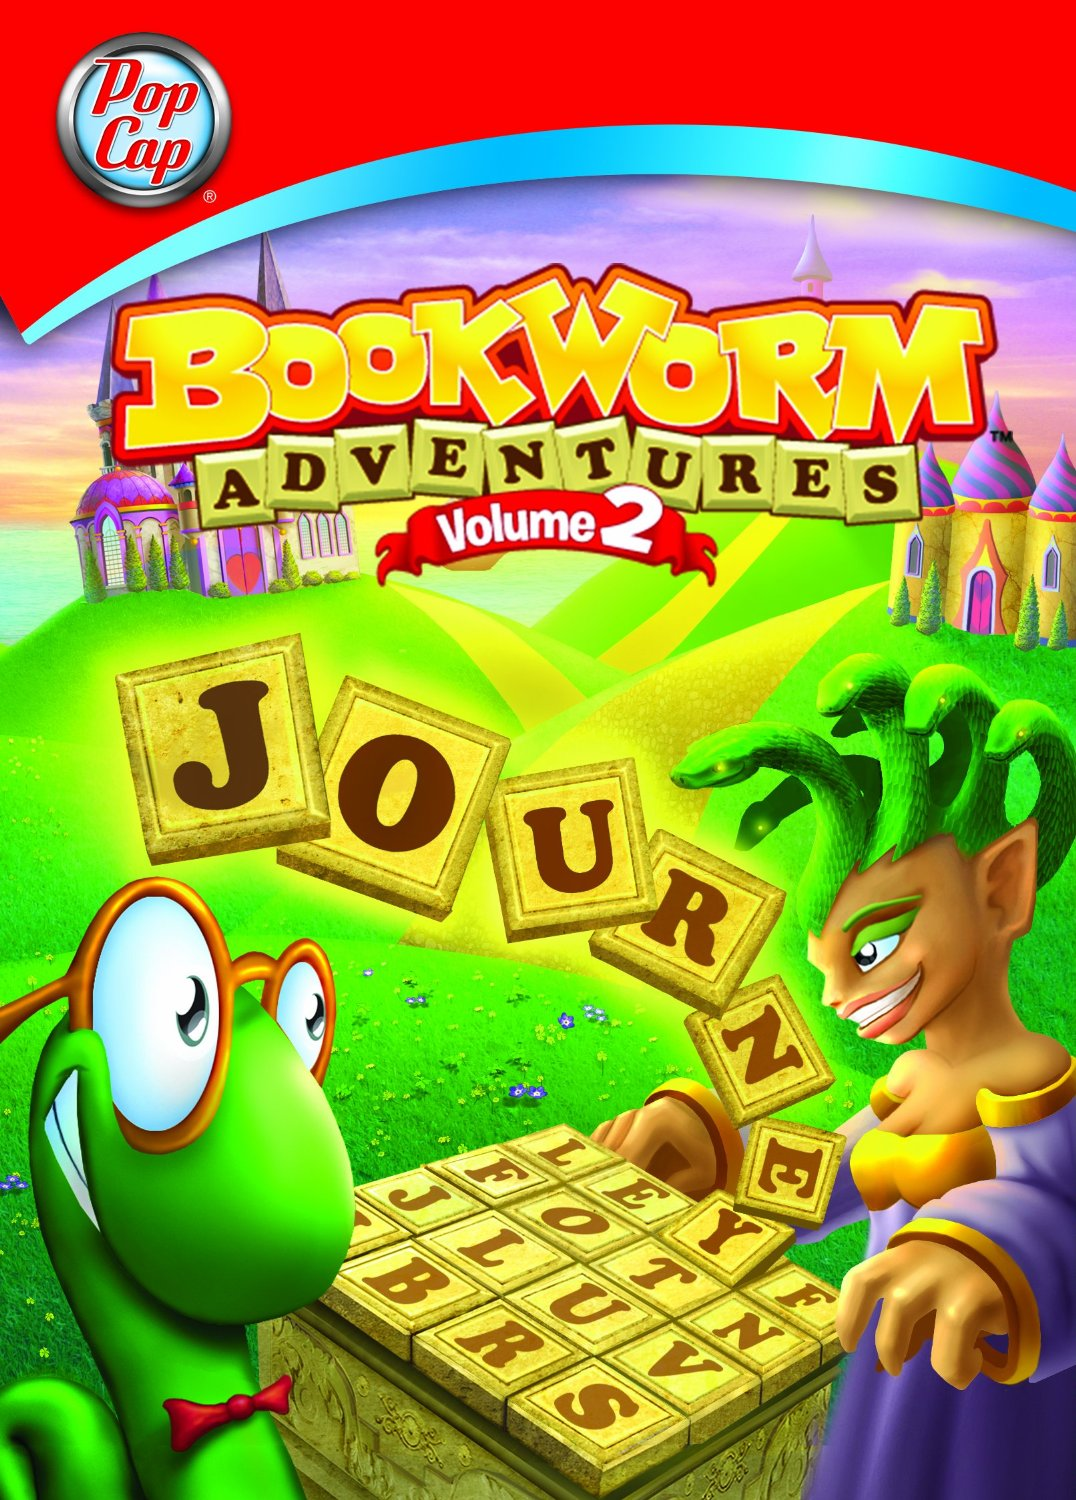
\includegraphics[width=.5\linewidth]{Images/bookworm.jpg}
  \vspace{0.5cm}
  \caption{Bookworm Adventures}
  \label{fig:test1}
\end{minipage}%
\begin{minipage}{.5\textwidth}
  \centering
  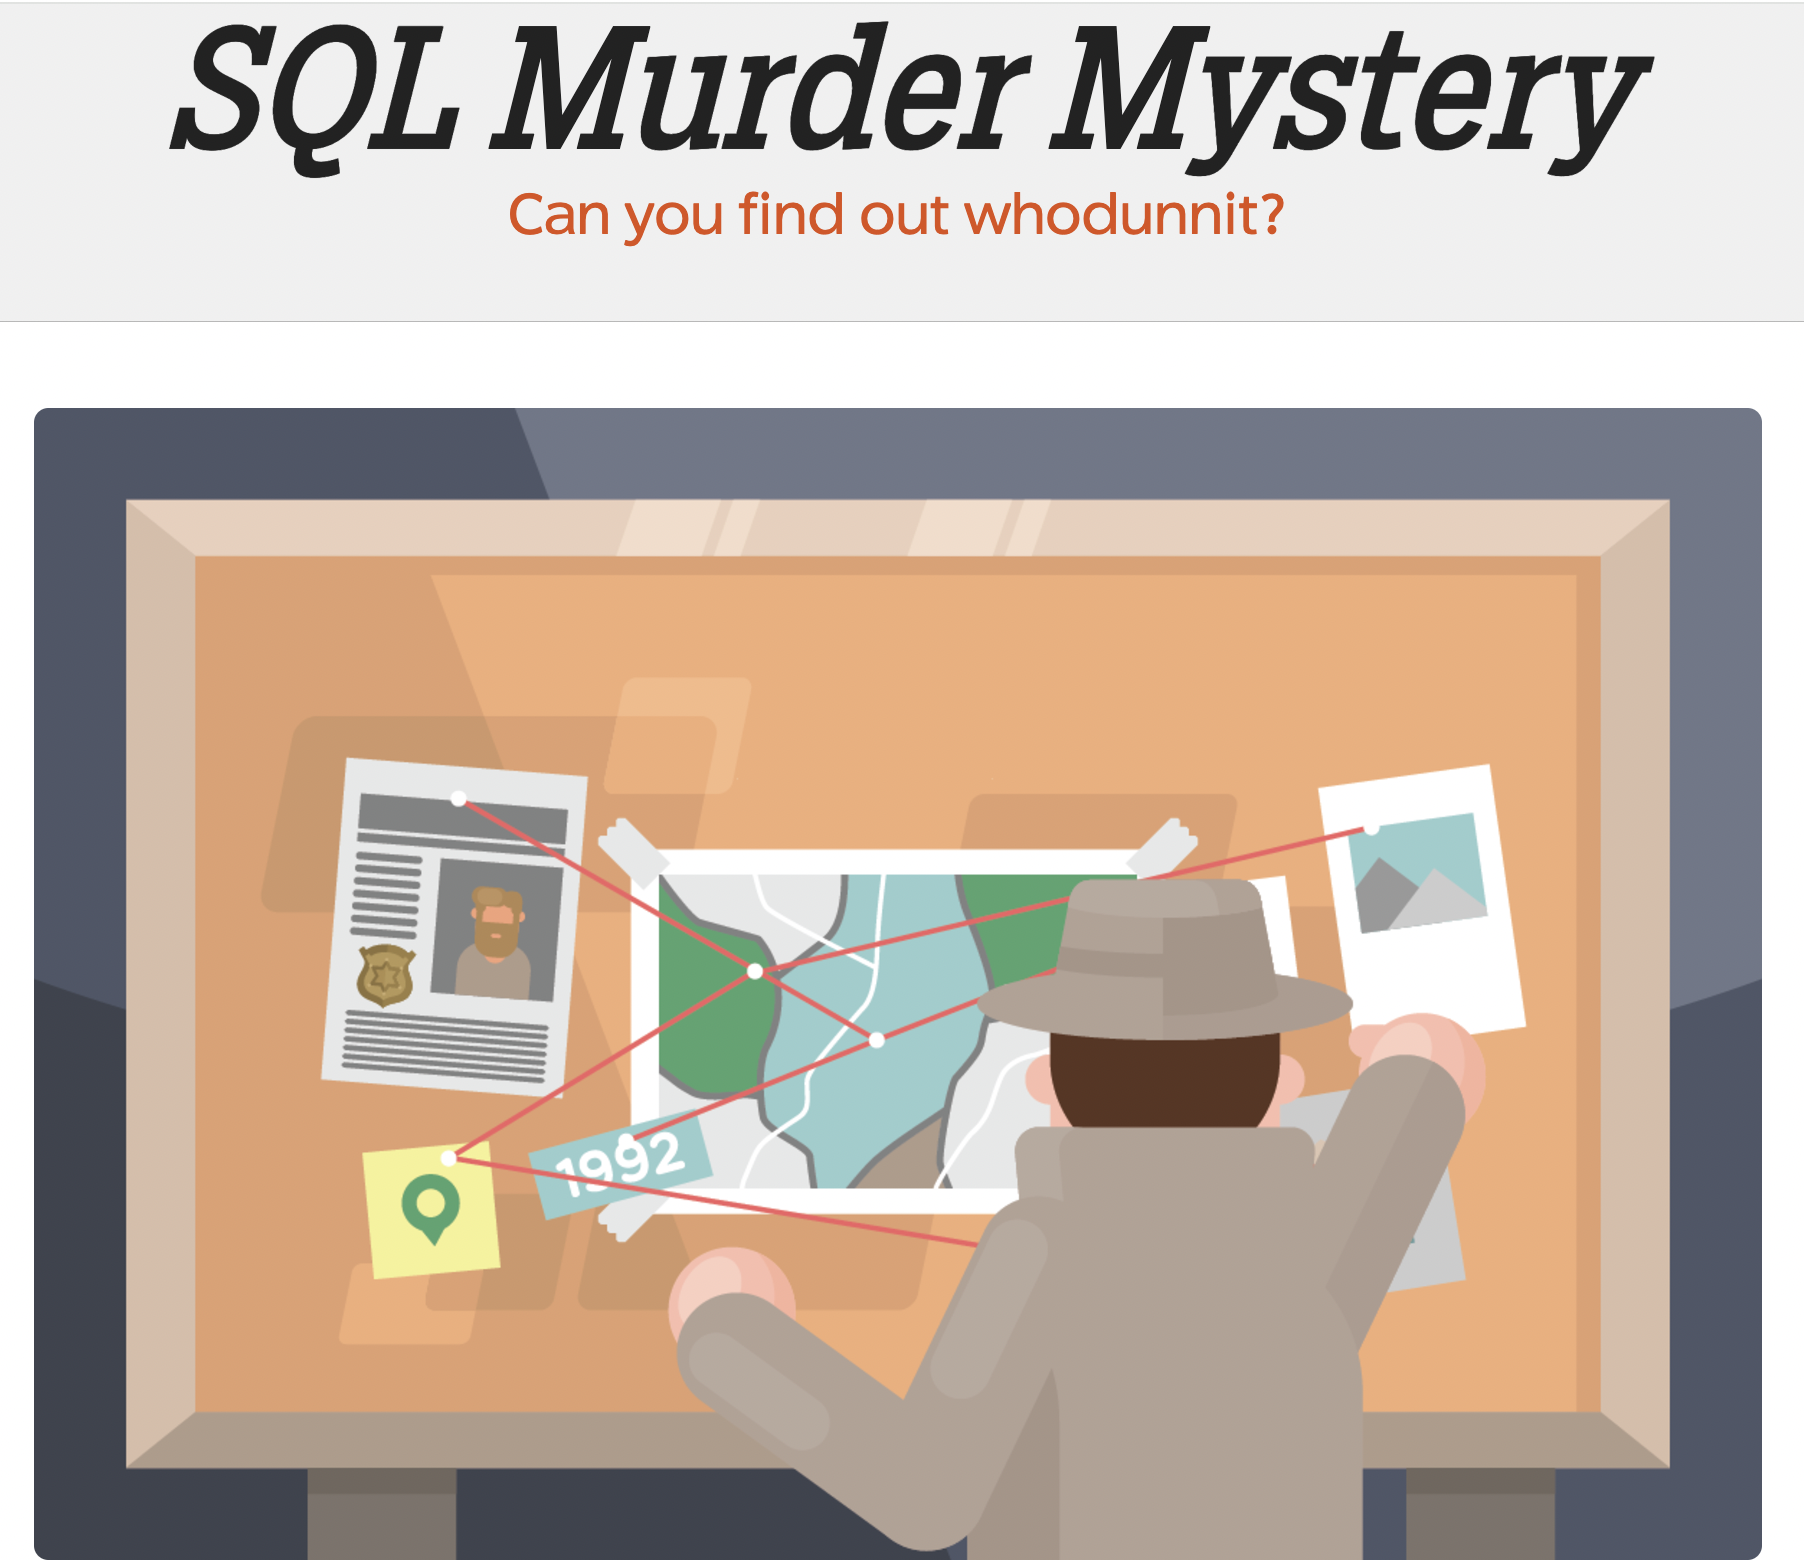
\includegraphics[width=.75\linewidth]{Images/SQL_murder.png}
  \vspace{0.5cm}
  \caption{SQL Murder Mystery}
  \label{fig:test2}
\end{minipage}
\end{figure}
\subsubsection{Bookworm Adventures}
\hspace*{0.5cm} Bookworm Adventures là một series game kết hợp giữa giải đố ghép chữ và yếu tố nhập vai chiến đấu. Người chơi điều khiển nhân vật chính, một chú sâu "mọt sách" Lex, trong hành trình phiêu lưu qua các thế giới thần thoại, đối đầu với quái vật và giải cứu bạn bè.\\
\hspace*{0.5cm} Người chơi sử dụng vốn từ vựng tiếng Anh để giúp Lex ghép các chữ cái trên màn hình thành các từ hợp lệ để tấn công quái vật bằng sức mạnh của từ ngữ. Từ càng dài và phức tạp thì sát thương gây ra càng cao.\\
\hspace*{0.5cm} Bookworm Adventures có hệ thống trang bị (mũ, vũ khí, phụ kiện) và dược phẩm để hỗ trợ Lex trong chiến đấu, ngoài ra còn có các chữ cái đặc biệt mang lại các hiệu ứng bổ sung (tăng sát thương, thiêu đốt, đóng băng..) khi được sử dụng để tạo từ.
\begin{figure}[H]
	\centering
	\includegraphics[width=0.75\textwidth]{Images/bookworm_play.png}
	\vspace{0.5cm}
	\caption{Tổng quan một màn chơi trong Bookworm Adventures}
\end{figure}
% \hspace*{0.5cm}
\subsubsection{SQL Murder Mystery}
\hspace*{0.5cm} SQL Murder Mystery là một trò chơi tương tác được thiết kế để giúp người chơi học và thực hành SQL thông qua việc giải quyết một vụ án bí ẩn. Chúng ta có thể chơi trực tuyến tại \textit{\def\UrlFont{\bfseries}\url{https://mystery.knightlab.com}}, trò chơi hoàn toàn miễn phí và không yêu cầu cài đặt bổ sung.\\
\hspace*{0.5cm} Trong trò chơi, chúng ta sẽ sử dụng kĩ năng SQL của bản thân để truy bắt kẻ sát nhân đang lẫn trốn trong thành phố SQL. Trò chơi bắt đầu bằng việc khám phá một vài bảng dữ liệu, và dần dần, bạn sẽ phát hiện ra các manh mối liên quan đến vụ án mạng. Ví dụ, ngay từ đầu, bạn tìm thấy một báo cáo của cảnh sát đề cập đến hai nhân chứng nhưng không xác định được nghi phạm. Sau đó, bạn thực hiện JOIN với bảng phỏng vấn nhân chứng, và dần dần tiến gần hơn đến việc xác định tên tội phạm.
\begin{figure}[H]
	\centering
	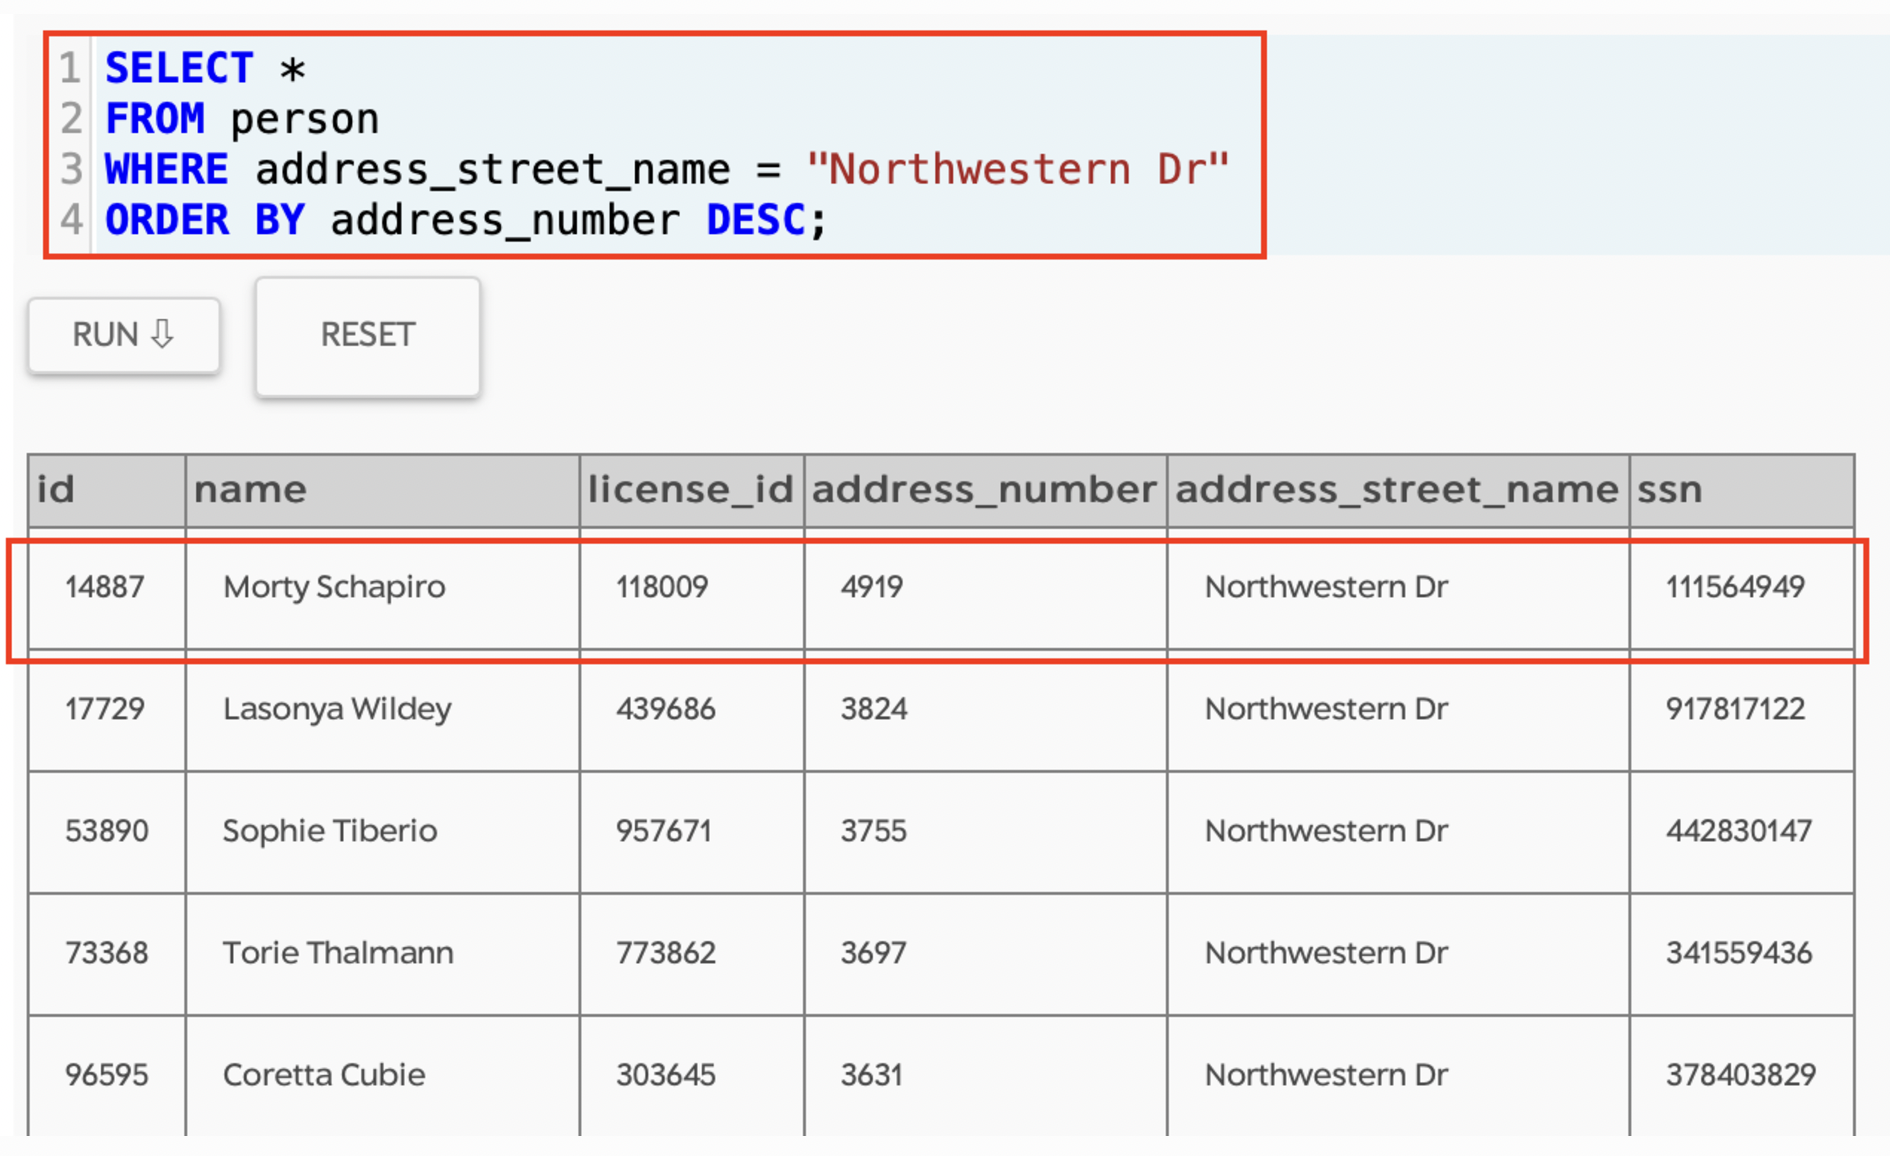
\includegraphics[width=0.75\textwidth]{Images/smm_play.png}
	\vspace{0.5cm}
	\caption{Tổng quan một câu truy vấn trong SQL Murder Mystery}
\end{figure}
\hspace*{0.5cm} Sau khi bắt được tên sát nhân ta nhận ra rằng hắn không phải kẻ chủ mưu thật sự. Các thám tử lại tiếp tục lên đường đi tìm tên thủ phạm đứng sau tất cả để trả lại trật tự cho thành phố SQL.
\begin{figure}[H]
\centering
\begin{minipage}{.5\textwidth}
  \centering
  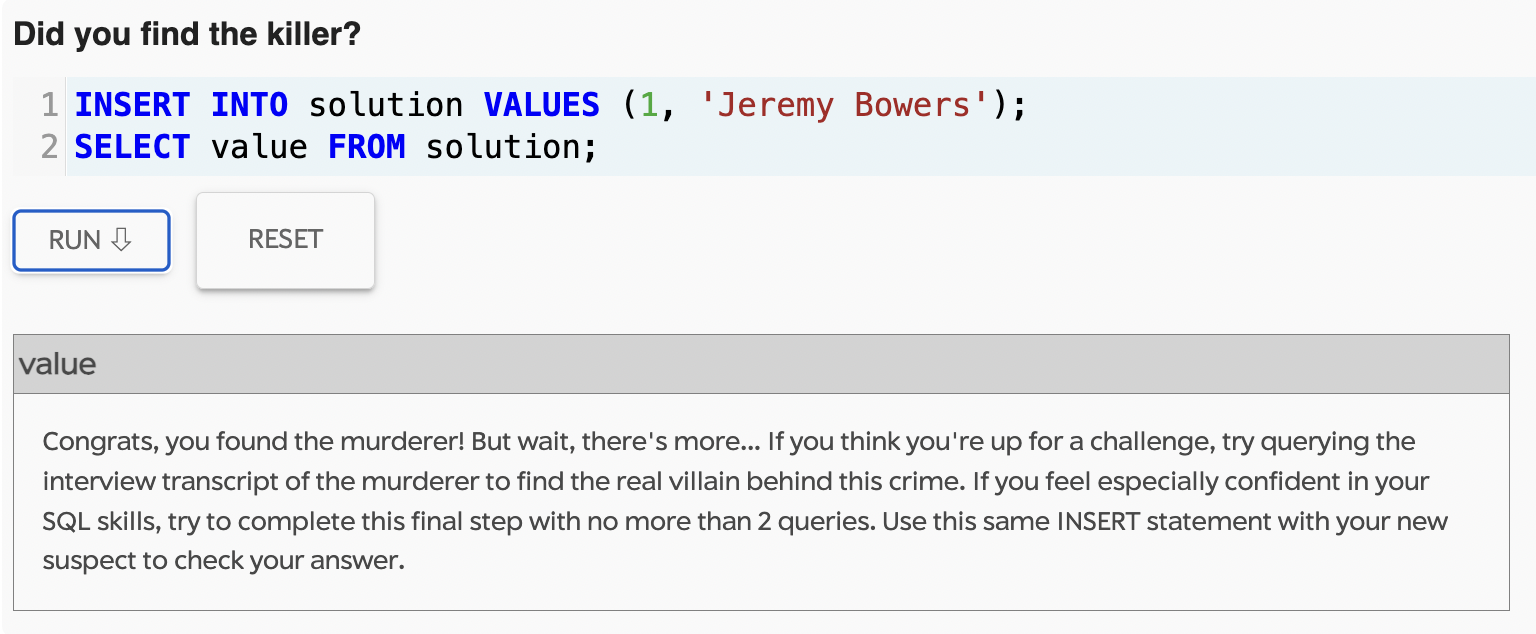
\includegraphics[width=0.75\linewidth]{Images/smm_killer.png}
  \vspace{0.5cm}
  \caption{Tìm ra kẻ sát nhân}
  \label{fig:test1}
\end{minipage}%
\begin{minipage}{.5\textwidth}
  \centering
  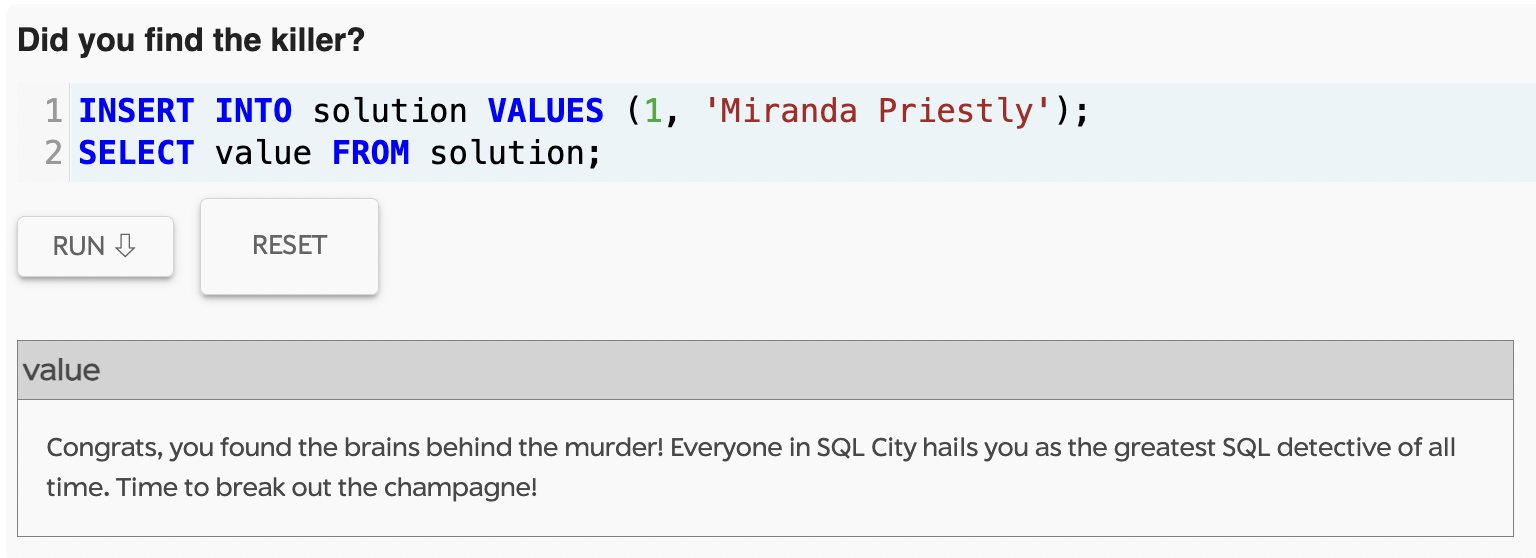
\includegraphics[width=.75\linewidth]{Images/smm_boss.png}
  \vspace{0.5cm}
  \caption{Tìm ra kẻ chủ mưu}
  \label{fig:test2}
\end{minipage}
\end{figure}
\hspace*{0.5cm} Trò chơi này đã nhanh chóng trở nên phổ biến nhờ cách tiếp cận sáng tạo và thú vị trong việc học lập trình SQL. Tuy nhiên, đồ hoạ của trò chơi vô cùng đơn giản, chỉ hiển thị kết quả của câu lệnh, không có hiệu ứng hay sự tương tác giữa game với người chơi. Nội dung của trò chơi cũng bị giới hạn quanh nhiềm vụ truy tìm thủ phạm, tính replay thấp.
\subsubsection{Điểm khác biệt của MeowSQL Knight}
\hspace*{0.5cm} Để MeowSQL Knight có thể tồn tài trên thị trường game, chúng ta cần khiến trò chơi có sự cải tiến hoặc một nét riêng để thu hút người chơi. Thông qua việc học tập, khắc phục những yếu điểm mà Bookworm Adventures và SQL Murder Mystery mắc phải và phát triển những tính năng mới. Trò chơi sẽ trở nên độc đáo, thu hút được một tập người chơi lớn hơn.\\
\hspace*{0.5cm} Đồ án kết hợp sử dụng ngôn ngữ truy vấn SQL vào chiến đấu theo lượt. Đồ án có giao diện Gameplay chính và xu hướng đồ hoạ slide scrolling giống với Bookworm Adventures. Trò chơi cũng có cốt truyện tập trung vào phiêu lưu và chiến đấu, song cách chơi lại lấy ý tưởng từ SQL Murder Mystery. Trò chơi sử dụng SQL là phương thức tương tác chính, người chơi sử dụng SQL để khai thác một schema đã cho, lấy thông tin về các điểm yếu của quái vật và tấn công chúng.\\
\hspace*{0.5cm} MeowSQL Knight hướng đến đa dạng đối tượng, tập trung chủ yếu vào học sinh cấp 3, sinh viên đại học đang học và thực hành SQL. Trò chơi sở hữu lối chơi vẫn mới mẻ với nhiều người, dễ dàng thu hút người chơi, ngoài ra với cốt truyện phân nhánh và thách thức trong việc đánh bại các quái vật sẽ làm tăng trải nghiệm của người chơi.


\subsection{Luật chơi Gameplay chính}
\hspace*{0.5cm} Mỗi màn chơi, người chơi sẽ được đưa đến một bản đồ, bao gồm các phòng liên thông với nhau. Nhiệm vụ của người chơi là khám phá các phòng, sử dụng các câu truy vấn để nhân vật chính tương tác với cắc đối tượng trong phòng chơi, hoàn thành yêu cầu được đưa ra trong mỗi căn phòng, đến điểm cuối của màn chơi và hoàn thành màn chơi.

\subsubsection{Bản đồ trong màn chơi}
\hspace*{0.5cm} Một màn chơi sẽ có dạng dungeon (hầm ngục) gồm nhiều phòng, mỗi phòng có thể liên thông 1 chiều với nhau (có lối đi từ phòng này sang phòng khác nhưng không thể đi ngược lại). Người chơi khi bắt đầu màn chơi sẽ bắt đầu ở căn phòng lối vào và kết thúc ở căn phòng lối ra. Chỉ có một lối vào và có một lối ra duy nhất. Ở lối ra thường sẽ có một Miniboss hoặc Boss trong đó. Các phòng bị bóng tối che khuất, chỉ có thể thấy các căn phòng lân cận (có lối đi từ phòng hiện tại) khi đã clear được căn phòng hiện tại.\\

\begin{figure}[H]
	\centering
	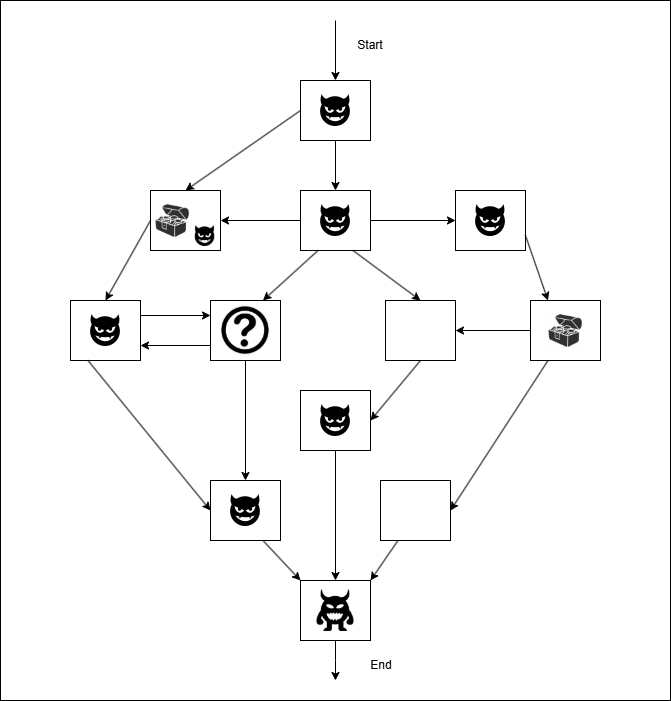
\includegraphics[width=10cm]{Images/SampleLevel.png}
	\vspace{0.5cm}
	\caption{Cấu trúc một bản đồ chơi}
\end{figure}

\hspace*{0.5cm}Trong một căn phòng, có thể xuất hiện quái vật, rương kho báu hoặc không có gì, đi cùng với một môi trường nhất định. Người chơi có thể chinh phục 1 căn phòng bằng các cách như tiêu diệt quái vật, mở rương kho báu hoặc đi vào 1 căn phòng trống. Sau khi chinh phục một căn phòng thì game sẽ mở khóa các căn phòng lân cận (không cần các phòng phải lối đi từ căn phòng hiện tại), người chơi quyết định đi căn phòng nào tiếp theo. Lưu ý rằng người chơi không được quay đầu (quay trở lại căn phòng đã đi trước đó). Các căn phòng có thể chứa các route đến các màn chơi khác trên bản đồ. Căn phòng cuối cùng, chính là lối ra, trong đó sẽ có một con boss hoặc min boss. Nhiệm vụ của người chơi là đánh bại boss đó để có thể thoát ra ngoài.\\
\subsubsection{Chiến đấu}
\hspace*{0.5cm}Gameplay chính của phần chiến đấu hoạt động theo dạng đánh theo lượt luân phiên giữa người chơi và quái vật.

\begin{itemize}
	\item Khi đến lượt của mình, người chơi được thực thi một câu lệnh hợp lệ của SQL. Câu lệnh phải chạy được thì mới tính là một câu lệnh hợp lệ. Để tấn công quái vật hoặc sử dụng vật phẩm, người chơi phải dùng câu \textbf{insert} để chèn các tham số vào các bảng mang chức năng đặc biệt. Mặc dù có cơ chế đánh theo lượt luân phiên, vẫn có khả năng người chơi sau khi xong một lượt có thể chơi một lượt nữa (đây gọi là sự nhanh nhẹn, nó sẽ là một chỉ số có ảnh hưởng đến xác suất đánh thêm lượt nữa của đối tượng đang ở lượt của mình). Điều này được tính cho cả người chơi và quái vật. Tuỳ hành động người chơi hoặc quái vật thực hiện mà xác suất thêm lượt cũng sẽ khác nhau.
	\item Đến lượt của quái, một lần duy nhất trong lượt quái vật có thể tấn công người chơi bằng tay không, hoặc sử dụng kỹ năng để tấn công hoặc áp dụng lên bản thân chúng. Đòn tấn công này có thể mang một số hiệu ứng khác nhau, tuỳ thuộc vào mức độ kháng hiệu ứng mà người chơi có thể chịu được hay không.
\end{itemize}

\subsubsection{Cơ chế đánh theo lượt}
\hspace*{0.5cm} Khi bắt đầu quá trình chiến đấu, việc quyết định phe nào đi trước được quyết định bằng một phép random với dải giá trị bao gồm điểm nhanh nhẹn của các thực thể tham gia chiến đấu, nếu random vào dải giá trị của đối tượng nào thì đối tượng đó được phép đi trước. Thứ tự đi của các thực thể được quyết định theo thứ tự độ nhanh nhẹn giảm dần và đi theo vòng tròn. Mỗi thực thể sẽ được cấp một chỉ số gọi là EnergyIndex với giá trị ban đầu là độ nhanh nhẹn của thực thể đó. Mỗi lần trong lượt, đòn tấn công của quái vật (thường) và của người chơi (tay không, sử dụng vũ khí trang bị) tiêu tốn 50\% độ nhanh nhẹn trừ vào EnergyIndex. Riêng các kỹ năng có thể tiêu tốn một lượng Energy Index yêu cầu để có thể ra chiêu. Người chơi nếu thực hiện truy vấn (trừ việc insert vào các bảng hành động) thì nó tiêu tốn 25\% lượng EnergyIndex hiện tại. Nếu Energy Index về 0 hoặc thấp hơn thì lượt tới sẽ là lượt của thực thể tiếp theo, ngược lại, việc quyết định lượt tiếp theo là của mình hay sẽ là của người khác sẽ phụ thuộc vào random tiếp với dải giá trị bao gồm Energy Index còn lại của các thực thể tham gia chiến đấu, bao gồm người chơi. Nếu lượt tiếp theo là lượt của đối phương thì Enengy Index sẽ reset về chỉ số nhanh nhẹn (chưa tính trường hợp dính hiệu ứng độc, làm chậm, băng). Khi đến lượt của người chơi, nếu TC < 0 (do hiệu ứng băng) thì người chơi không thể thao tác và chuyển đến cuối lượt người chơi (nơi sẽ áp dụng hiệu ứng)\\
\hspace*{0.5cm} Cấu trúc của một lượt của đối tượng được chia thành nhiều giai đoạn, cụ thể như sau. 
\begin{figure}[H]
	\centering	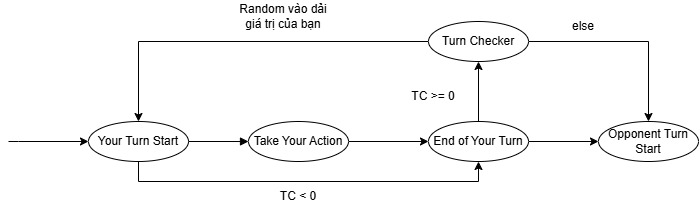
\includegraphics[width=\textwidth]{Images/turnphases.jpg}
	\vspace{0.5cm}
	\caption{Các giai đoạn trong lượt trong đối tượng (người chơi/quái vật)}
\end{figure}
\begin{itemize}
	\item \textbf{Turn Start}: bắt đầu của lượt, ở giai đoạn này game sẽ kiểm tra xem trạng thái Energy Index của bạn có lớn hơn 0 hay không, nếu không thì phải chuyển đến giai đoạn cuối của lượt.
	\item \textbf{Take Action}: giai đoạn chính của lượt chơi, nơi các hành động của người chơi/quái vật sẽ được thực thi. Ứng với mọi hành động mà EnergyIndex cũng sẽ tiêu hao.
	\item \textbf{End of Turn}: giai đoạn kết thúc của lượt, tại giai đoạn này các hiệu ứng người chơi đang mắc phải sẽ gây ảnh hưởng đến người chơi (ví dụ như hiệu ứng lửa sẽ đốt người chơi gây mất máu) và sau đó các trạng thái hiệu ứng sẽ giảm một lượng bằng chỉ số kháng hiệu ứng. Sau đó Energy Index sẽ được kiểm tra xem TC còn >= 0, nếu không thì sẽ chuyển sang lượt đối thủ và chỉ số được reset (bao gồm cả ảnh hưởng các hiệu ứng nếu còn).
	\item \textbf{Turn Checker}: nếu EnergyIndex >= 0 tại End of Turn thì sẽ chuyển sang giai đoạn Turn Checker. Controller sẽ quyết định lượt tiếp theo là của mình hay của người khác bằng giá trị random trên dải giá trị bao gồm Energy Index còn lại của mình và đối thủ. Nếu giá trị thuộc dải của mình thì sẽ đến lượt mới với giai đoạn bắt đầu lượt của mình. Nếu không thì sẽ chuyển sang lượt đối thủ và đặt lại giá trị Energy Index được reset (bao gồm cả ảnh hưởng các hiệu ứng nếu còn) 
\end{itemize}
\subsubsection{Mã định danh}
\hspace*{0.5cm} Với một màn chơi, người chơi, quái vật, các bộ phận của quái vật và các vật thể môi trường sẽ được nằm chung một bảng \textbf{Entities} có khoá là một mã EntityID có cùng một định dạng, cấu trúc. Đây là chuỗi ký tự có độ dài 8 ký tự cố định (gồm số, chữ in thường). Mỗi EntityID chỉ được sở hữu bởi nhiều nhất 1 object. Khi Object chết và màn chơi tiếp tục, EntityID này sẽ được thu hồi và nó không còn tồn tại với bất kỳ hình thức nào.
\hspace*{0.5cm} Ngoài mã định danh thực thể còn có mã định danh vật phẩm, gồm một chuỗi có 7 ký tự. Mã định danh kỹ năng gồm 6 ký tự, bao gồm chữ số, ký tự thường.
\subsubsection{Thực thể}
\hspace*{0.5cm} Người chơi, quái vật, bộ phận chí mạng của quái vật sẽ có chung một bảng trong cơ sở dữ liệu để lưu trữ các thông tin của thực thể, các thuộc tính trong bảng bao gồm:\\
\begin{itemize}
	\item \textbf{Mã định danh thực thể EntityID}
	\item \textbf{Tên thực thể}
	\item \textbf{Mô tả thực thể}
	\item \textbf{Loại thực thể}: có thể là người chơi, quái vật, bộ phận chí mạng,...
	\item \textbf{Mã thực thể là cha của của thực thể}: Thuộc tính này được sử dụng đối với bộ phận chí mạng của quái vật. còn lại thì giá trị này là null.
	\item \textbf{Máu hiện tại}
	\item \textbf{Máu tối đa hiện tại}
	\item \textbf{Level của thực thể}: đối với bộ phận thì level mặc định sẽ là 0
	\item \textbf{Chỉ số Energy Index}
	\item \textbf{Các trạng thái hiệu ứng thực thể dính phải}: bao gồm lửa, băng, độc và mù.
	\item \textbf{Các traits hiện tại của thực thể}: Đối với người chơi, trait này được tổng hợp từ trang bị thủ. Đối với quái vật và bộ phận chí mạng là từ Chủng loại quái vật.
\end{itemize}

\subsubsection{Người chơi}
\hspace*{0.5cm} Người chơi sử dụng bảng \textbf{Entities} để lưu trữ các thông tin của người chơi. Ngoài ra, người chơi được cung cấp một số lượng slot trang bị nhất định, người chơi trang bị vũ khí và giáp vào các slot này, mỗi slot chỉ được chứa một trang bị. Các trang bị sẽ được kích hoạt các chỉ số và hiệu ứng phụ trợ khi đã được trang bị. Người chơi cũng sẽ có môt inventory để chứa các vật phẩm có thể sử dụng trong chiến đấu.\\

\subsubsection{Cơ chế kho đồ/vật phẩm/trang bị}
\hspace*{0.5cm} Thứ cần thiết cho game không thể thiếu là các vật phẩm, các trang bị sẽ hỗ trợ người chơi trên chuyến hành trình. Các vật phẩm có thể có nhiều cách thu thập khác nhau:
\begin{itemize}
	\item Thu thập khi mở rương trong màn chơi
	\item Thu thập qua đánh boss
	\item Mua bán, trao đổi
	\item Mở rương kho báu
\end{itemize}

\hspace*{0.5cm} Các vật phẩm có thể là trang bị, vật phẩm sử dụng được cũng như không phải cả 2 loại trên. Điểm chung của các loại vật phẩm này là các vật phẩm sẽ mang một ID riêng biệt cho từng vật phẩm, cấu trúc mã định danh vật phẩm, gồm một chuỗi có 7 ký tự, bao gồm chữ số và ký tự thường. Mã định danh này là cố định xuyên suốt toàn bộ quá trình của game và không thể thay đổi được.\\

\textbf{Phân cấp theo độ hiếm}
\hspace*{0.5cm} Có thể phân chia độ hiếm của trang bị thành các phân cấp như sau:
\begin{itemize}
	\item Common - 1 sao
	\item Uncommon - 2 sao
	\item Rare - 3 sao
	\item Myth - 4 sao
	\item Legendary - 5 sao
\end{itemize}

\hspace*{0.5cm} Mỗi phân cấp khác nhau sẽ mở khóa tiềm năng vật phẩm khác nhau, bao gồm hiệu quả sử dụng, chỉ số cơ bản, chỉ số nâng lên mỗi cấp, số lượng trait và các trait chất lượng,... Độ hiếm càng cao giới hạn chỉ số càng lớn, ngoài ra còn đi kèm các hiệu ứng mạnh hơn, cũng như nhiều traits hơn (nhưng với mọi trang bị, giới hạn tối đa là 5 traits)\\

\hspace*{0.5cm} Độ hiếm vật phẩm càng cao, hiệu quả sử dụng của vật phẩm càng lớn, song giá mua cao hoặc khó tìm hơn. 
\hspace*{0.5cm} Vật phẩm tiêu thụ được là các vật phẩm có thể sử dụng được trong chiến đấu. Vật thể tiêu thụ được có thể hồi máu, tăng độ nhanh nhẹn, tấn công, phòng thủ của người sử dụng, các chỉ số này sẽ được cộng vào và có hiệu lực ngay lập tức cho đến khi kết thúc chiến đấu, ngoài ra còn có tác dụng giải hiệu ứng một lượng tương ứng với từng loại hiệu ứng khác nhau.\\


\textbf{Trang bị}
\hspace*{0.5cm} Trang bị vũ khí và trang bị giáp đều sử dụng một bảng \textbf{Equipment} để lưu trữ thông tin trang bị trong schema. Trang bị mang một bộ chỉ số cố định, người chơi có thể sử dụng trang bị để tấn công, có thể sử dụng vũ khí hay giáp đều sử dụng được.\\

\hspace*{0.5cm} Dữ liệu trang bị bao gồm:\\
\begin{itemize}
	\item \textbf{Mã định danh trang bị}: gồm chuỗi 7 kí tự, bao gồm chữ thường và số
	\item \textbf{Tên trang bị}
	\item \textbf{Loại trang bị}: có thể là các loại sau:
	\begin{itemize}
		\item Vũ khí
		\begin{itemize}
			\item Vũ khí dùng để tấn công quái vật cho ra sát thương tốt nhất. Traits của vũ khí sẽ được sử dụng để xét mức độ hiệu quả đòn đánh dựa vào trait. Vũ khí không tính cộng dồn trait cho người chơi.
		\end{itemize}
		\item Giáp
		\begin{itemize}
			\item Khi quái vật tấn công vào giáp thì giáp sẽ phát huy hiệu quả khi ngăn cản đòn đánh của quái vật cũng như có thể kháng hiệu ứng. Người chơi vẫn có thể tấn công quái vật bằng giáp được, nhưng sát thương của chúng thường rất nhỏ, tuy nhiên vẫn sử dụng trait để xét mức độ hiệu quả. Các trang bị giáp sẽ được tính tổng hợp trait cho người chơi.
		\end{itemize}
		\item Giày
		\begin{itemize}
			\item Giày có thể tăng chỉ số giáp và nhanh nhẹn, cũng như giáp, chỉ số tấn công gần như bằng 0 nên Khi quái vật tấn công vào thì giáp sẽ phát huy hiệu quả khi ngăn cản đòn đánh của quái vật cũng như có thể kháng hiệu ứng. Tương tự giáp, giày cũng sẽ được tính tổng hợp trait cho người chơi.
		\end{itemize}
	\end{itemize}
	\item \textbf{Mô tả}
	\item \textbf{Cấp độ hiện tại}
	\item \textbf{Cấp độ yêu cầu người chơi đạt được mới có thể sử dụng}
	\item \textbf{Tối đa 3 Trait}
\end{itemize}
\hspace*{0.5cm} Trang bị đều mang cùng bộ khung chỉ số với quái vật và người chơi, bao gồm chỉ số cơ bản, chỉ số hiện tại sau khi tính qua cấp độ của món trang bị, hệ số nâng cấp chỉ số giống với của người chơi và quái vật (sẽ đề cập trong các phần sau). Tuy nhiên khi hiển thị dữ liệu trên schema chỉ lấy chỉ số hiện tại để tránh gây khó khăn khi tra cứu.\\


\textbf{Vật phẩm/Kho đồ}
\hspace*{0.5cm} Các vật phẩm được hiển thị thông tin trong bảng \textbf{Inventory}. Bảng này được dùng để lưu trữ thông tin vật phẩm cũng như trạng thái của chúng trong kho đồ người chơi.\\

\hspace*{0.5cm} Dữ liệu của một vật phẩm được thể hiện bao gồm:\\
\begin{itemize}
	\item \textbf{Mã định danh vật phẩm}: gồm chuỗi 7 kí tự, bao gồm chữ thường và số
	\item \textbf{Tên vật phẩm}
	\item \textbf{Loại vật phẩm}: có thể là bình máu, bình giải hiệu ứng, bình tăng sức mạnh,...
	\item \textbf{Mô tả}
	\item \textbf{Số lượng hiện có}
	\item \textbf{Lượng máu hồi phục}
	\item \textbf{Sức tấn công được gia tăng}
	\item \textbf{Sức phòng thủ được gia tăng}
	\item \textbf{Độ nhanh nhẹn được gia tăng}
	\item \textbf{Lượng giải trừ hiệu ứng}: Độc, Băng, Lửa, Mù
\end{itemize}

\textbf{Cơ chế Kho đồ/ Slot trang bị}
\begin{itemize}
	\item Kho đồ trong game có không gian lưu trữ lớn, nhưng nó có giới hạn, chủ yếu lưu trữ các trang bị không sử dụng và các vật phẩm tiêu hao cùng vật phẩm khác. Khi người chơi chết thì tất cả các món đồ trong kho không bị ảnh hưởng. Với trang bị, người chơi chỉ có thể có số lượng một với mỗi trang bị trong kho đồ, nếu nhận thêm thì trang bị dư thừa sẽ chuyển sang đơn vị có giá trị tương đương
	\item Slot trang bị cho phép người chơi gán các trang bị vào để mang đi chiến đấu. Có tối đa 8 slot trang bị, ban đầu người chơi chỉ có 4 slot trang bị, có thể nâng cấp tại cửa hàng. Nếu người chơi chết, các món trang bị không bị mất, nhưng chúng sẽ bị giảm cấp độ (tùy dev tùy chỉnh mà có thể giảm ít, hay nhiều).
	\item Trong màn chơi, người chơi không được gán trang bị từ kho vào slot và ngược lại. Việc này chỉ được thực hiện bên ngoài bản đồ hay ở khu Safe Zone.
	\item Những món vật phẩm trong cơ sở dữ liệu trong màn chơi chính là các trang bị mang theo và các vật phẩm tiêu hao được nằm trong kho đồ của người chơi. 
\end{itemize}






\subsubsection{Kỹ năng (Skills)}
\begin{itemize}
	\item Người chơi và quái vật có cùng một bộ kỹ năng. Bộ kỹ năng này bao gồm nhiều kỹ năng mà người chơi có thể học được qua việc tăng cấp hoặc thu thập các cuộn kỹ năng. 
	\item Dữ liệu kỹ năng được lưu trữ trong bảng \textbf{Skills}. Dữ liệu của kỹ năng bao gồm:
	\begin{itemize}
		\item \textbf{Mã định danh kỹ năng}: gồm chuỗi 6 kí tự, bao gồm chữ thường và số. Mỗi mã định danh chỉ chứa 1 kỹ năng
		\item \textbf{Tên kỹ năng}
		\item \textbf{Mô tả}
		\item \textbf{Số lượt hồi lại sau khi sử dụng}
		\item \textbf{Năng lượng tiêu hao khi sử dụng}
		\item \textbf{2 traits}
	\end{itemize}
	\item Mỗi kỹ năng đều có chỉ số thay đổi. Khi được triển khai. Nó sẽ lấy chỉ số hiện tại của người chơi (đánh thường) cộng với chỉ số thay đổi của kỹ năng. Nếu là đòn tấn công thì sẽ áp dụng cả sát thương phép từ sát thương tiêu chuẩn nhân với hệ số sát thương phép. Nếu là kỹ năng hiệu ứng áp dụng cho bản thân thì sẽ được chuyển đổi các chỉ số tương ứng sang dạng hiệu ứng và cộng vào người thực thi. Nếu là quái vật sử dụng kỹ năng hồi máu thì máu sẽ được hồi cho bộ phận yếu máu nhất của quái vật. Tương tự với maxHP.
\end{itemize}

\subsubsection{Hiệu ứng}
\begin{itemize}
	\item \textbf{Độc}
	\begin{itemize}
		\item Gây sát thương: 5\% lượng máu tối đa khi hết lượt
		\item Giảm độ nhanh nhẹn: 40\%
	\end{itemize}
	\item \textbf{Lửa}
	\begin{itemize}
		\item Gây sát thương: 15\% lượng máu tối đa khi hết lượt
	\end{itemize}
	\item \textbf{Băng}
	\begin{itemize}
		\item Giảm độ nhanh nhẹn xuống -1
	\end{itemize}
	\item \textbf{Mù}
	\begin{itemize}
		\item Người chơi sẽ không nhìn được một số ô trong bảng với câu \texttt{SELECT}
	\end{itemize}
\end{itemize}
\textbf{Chỉ số kháng hiệu ứng}
\begin{itemize}
	\item Mỗi người chơi/quái vật sẽ có một bộ chỉ số kháng hiệu ứng nhất định.
	\item Khi tấn công đối phương, nếu kháng hiệu ứng tương ứng lớn hơn sát lực hiệu ứng, đối phương sẽ không dính hiệu ứng.
	\item Nếu kháng hiệu ứng nhỏ hơn sát lực hiệu ứng, đối phương sẽ chịu hiệu ứng với trạng thái (state) của hiệu ứng cộng thêm sát lực hiệu ứng đó trừ cho kháng hiệu ứng.
	\item Trước khi kết thúc lượt của đối tượng hiện tại, hiệu ứng sẽ gây ảnh hưởng người mắc (nếu có) và trạng thái hiệu ứng được trừ đi một lượng chỉ số bằng kháng hiệu ứng của người chơi. Nếu trạng thái hiệu ứng nhỏ hơn hoặc bằng 0, hiệu ứng sẽ kết thúc.
\end{itemize}
\textbf{Trang bị và sát lực hiệu ứng}
\begin{itemize}
	\item Chỉ số kháng hiệu ứng của người chơi được tổng hợp từ các trang bị giáp và giày trong slot.
	\item Mỗi món trang bị sẽ có một bộ sát lực riêng và không tính tổng hợp.
	\item Khi người chơi tấn công, sẽ tính chỉ số sát lực hiệu ứng trên món trang bị và kỹ năng (skill) được sử dụng để tấn công.
\end{itemize}

\textbf{Hiệu ứng trên quái vật}
\begin{itemize}
	\item Quái vật sẽ chịu hiệu ứng trên bản thể của quái vật.
	\item Hiệu ứng sẽ gây sát thương lên bộ phận ngẫu nhiên của quái vật.
\end{itemize}
\subsubsection{Bộ chỉ số}
\hspace*{0.5cm} Bộ chỉ số được sử dụng chung giữa các món trang bị, kỹ năng, người chơi, quái vật với các mục đích của bộ chỉ số là khác nhau. Dữ liệu chỉ số được lưu trên bảng \textbf{Stat}. Cấu trúc của bộ chỉ số bao gồm:
\begin{itemize}
	\item \textbf{Mã định danh chủ sỡ hữu}.
	\item \textbf{Loại chỉ số}: Có thể là chỉ số cơ bản, chỉ số hiện tại,... 
	\item \textbf{Tấn công}.
	\item \textbf{Phòng thủ}.
	\item \textbf{Nhanh nhẹn}.
	\item \textbf{Hệ số khuếch đại sát thương phép}.
	\item \textbf{Tỉ lệ chí mạng}: Khi tấn công kẻ địch, sẽ kiểm tra xem đòn đánh có phải là chí mạng không, dựa vào tỉ lệ này.
	\item \textbf{Hệ số khuếch đại chí mạng}: trong trường hợp nếu là chí mạng, thì sát thương sẽ được nhân với hệ số khuếch đại chí mạng. Con số này có thể lơn hơn 1 (hoặc cũng có thể nhỏ hơn 1).
	\item \textbf{Hút máu}: Hệ số tỉ lệ hút máu dựa vào sát thương sau khi trừ giáp (thấp nhất là 0 và cao nhất là 1)
	\item \textbf{Thay đổi HP}: Số HP bị cộng vào hoặc trừ bớt đi.
	\item \textbf{Bộ thông số sát thương hiệu ứng}: bao gồm hiệu ứng, lửa, băng, độc và mù.
	\item \textbf{Bộ thông số kháng hiệu ứng}: gồm các hiệu ứng tương tự với sát thương hiệu ứng.
\end{itemize}
\hspace*{0.5cm} Trong trường hợp nếu là kỹ năng hiệu ứng áp dụng cho bản thân người thi triển thì chỉ số thay đổi sẽ được chuyển đổi như sau:
\begin{itemize}
	\item \textbf{Thay đổi HP} -> \textbf{Hồi máu}
	\item \textbf{Tấn công} -> \textbf{Nâng cấp sức mạnh tấn công}
	\item \textbf{Phòng thủ} -> \textbf{Nâng cấp sức mạnh phòng thủ}
	\item \textbf{Nhanh nhẹn} -> \textbf{Tăng độ nhanh nhẹn}
	\item \textbf{Bộ thông số kháng hiệu ứng} -> \textbf{Giải trừ hiệu ứng}
\end{itemize}
\hspace*{0.5cm} Bộ thông số đã chuyển đổi này cũng được sử dụng khi người chơi sử dụng vật phẩm tiêu hao.

\subsubsection{Trait System}
\hspace*{0.5cm} Có một bộ các Trait (phẩm chất/hệ) được sử dụng chung bởi các thực thể và trang bị. Mỗi object nói trên sẽ có một số lượng trait nhất định.\\
\hspace*{0.5cm} Trong hệ thống trait, Một trait có thể bị một hoặc nhiều trait khác khắc chế, hoặc một trait có thể khắc chế nhiều trait khác, cũng có thể không bị khắc chế hay khắc chế trait nào. Số lượng trait khắc chế không được vượt quá một ngưỡng nào đó, nhưng không phải số lượng trait khắc chế của mỗi trait là bằng nhau. Có thể có một số trait khắc chế ít, nhưng dễ xuất hiện trong các trang bị, kỹ năng, quái vật. Nhưng cũng có trait khắc chế nhiều traits khác. Nhưng nó thưởng ở các trang bị, kỹ năng hiếm, cũng như là ở các Boss.\\ 
\hspace*{0.5cm} Quái vật lựa chọn trait từ danh sách trait chủng loại quái vật đang có. Các kỹ năng của chủng loại quái vật cũng phải tuân thủ có ít nhất một trait thuộc chủng loại. Người chơi tổng hợp trait từ các trang bị giáp và giày, vũ khí không được tổng hợp nhưng sử dụng traits khi tấn công.\\
\hspace*{0.5cm} Khi tấn công, bên tấn công và bên bị tấn công sẽ tiến hành so sánh trait được chọn để tấn công (ví dụ như là bên tấn công bằng vũ khí thì trait sẽ là của vũ khí đó, còn bên bị tấn công sẽ là các trait được lựa chọn, tổng hợp). Số điểm từ bộ trait mỗi bên được tính bằng tổng số cặp trait (A,B) mà mỗi trait A bên này là khắc chế của B bên kia. Nếu số điểm phe tấn công cao hơn bên bị tấn công thì sát thương sẽ được khuếch đại, ngược lại nếu phe tấn công thấp hơn phe bị tấn công thì sát thương sẽ bị giảm. Những phản ứng như thế này sẽ được thông báo đến người chơi sau mỗi đòn đánh.\\



\subsubsection{Quái vật}
\hspace*{0.5cm} Tương tự người chơi quái vật cũng lưu trữ các thông tin của mình trong bảng \textbf{Entities} trong Schema. Các quái vật vẫn mang các chỉ số thuộc tính và trait tương tự người chơi, chỉ có điều Traits được lấy từ chủng loại quái vật. Chỉ số máu và máu tối đa không còn quan trọng nữa, vì nó không tồn tại nhờ HP mà nhờ vào các bộ phận của nó. Quái vật có thể tấn công thường, sử dụng kỹ năng hoặc không tấn công. Quái vật cũng mang một số kỹ năng, cũng như sử dụng chung bảng trạng thái kỹ năng hiện tại với người chơi.\\

\hspace*{0.5cm} Ngoài ra có một bảng \textbf{Knowledge} cung cấp các gợi ý giúp cho người chơi có thể đánh bại quái vật. Tuy nhiên những gợi ý này có thể đúng hoặc có thể sai. Vì vậy người chơi cần phân tích kỹ để đưa ra quyết định đúng.\\
\paragraph{Chủng loại quái vật}
\hspace{0.5cm} Mỗi quái vật sẽ mang một chủng loại nhất định, trong loại quái vật có tên và mô tả quái vật và có một bộ trait tương ứng với từng loại. Quái vật có thể chọn một hoặc nhiều trait làm trait khi tấn công thường, và một số trait làm trait của bộ phận (không nhất thiết phải chọn toàn bộ trait thuộc loại quái vật). Ngoài ra chủng loại quái vật cũng có bộ kỹ năng nhất định cho từng loại, những thành phần kỹ năng tương tự với của người chơi, tuy nhiên kỹ năng được xem là kỹ năng của chủng loại quái vật khi có ít nhất 1 trait thuộc trait của chủng loại của quái vật. Quái vật có thể lựa chọn 1 số kỹ năng, không nhất thiết phải toàn bộ. Nhiều loại quái vật có thể có cùng một kỹ năng, sẽ có các kỹ năng độc quyền của quái vật, có thể liên quan đến chiến đấu hoặc cũng có thể liên quan đến SQL, đặt ra các tình huống để người chơi sử dụng kiến thức SQL để giải quyết. Khi đến lượt của quái, quái sẽ chọn đòn đánh thường hoặc một kỹ năng ngẫu nhiên đủ điều kiện (đã hồi chiêu xong và đủ năng lượng thực thi) và thi triển, kỹ năng nó cũng sẽ mất một khoảng thời gian để phục hồi. Có một xác suất quái vật ngủ, không tấn công người chơi.\\

\paragraph{Bộ phận chí mạng của quái vật}
\hspace*{0.5cm} Quái sẽ không sống nhờ HP, mà chúng sẽ sống nhờ vào các bộ phận chí mạng trên cơ thể, Tình trạng sống/chết của quái vật phụ thuộc vào tình trạng tồn tại của các bộ phận này. Nếu mất hết tất cả bộ phận chí mạng, quái sẽ chết. \\
\hspace*{0.5cm} Các bộ phận nằm trên cơ thể và có bộ dữ liệu nằm chung bảng \textbf{Entities} với Quái vật và người chơi. Thông tin một bộ phận sẽ là một bảng ghi chứa thông tin chung của tất cả bộ phận quái vật với \textit{parentID} thuộc quái vật hoặc là null. Quái vật có thể có một số lượng bộ phận nhất định. Khi người chơi tấn công vào các bộ phận này sẽ phải chịu giáp và kháng hiệu ứng của quái vật, rồi mới trừ vào máu của bộ phận, hiệu ứng sẽ áp dụng cho quái vật, người chơi vẫn tấn công vào EntityID của quái vật bình thường, nhưng hoàn toàn vô dụng, cả sát thương và hiệu ứng đều sẽ không áp dụng cho quái vật.\\ Một số đặc điểm của một bộ phận. \\

\subsubsection{Dữ liệu giả của quái vật}
\hspace*{0.5cm} Trong chiến đấu, có thể sẽ có các dữ liệu của quái vật hoặc bộ phận quái vật là dữ liệu giả. Những dữ liệu này được chúng tạo ra khi bắt đầu chiến đấu hoặc sử dụng kỹ năng trong khi chiến đấu\\
\hspace*{0.5cm} Các bản sao của quái vật không có khả năng tạo các bản sao. Các cấu trúc về đặc điểm của bản thật sẽ được sao chép sang bản sao. TUY NHIÊN, một số bản sao có thể có sự khác biệt với bản thật ở một số điểm, một số thông số,.... Bản sao sẽ lựa chọn một giá trị ngẫu nhiên trên dải giá trị để làm giá trị cho mình. Bản sao có thể lựa chọn chủng loại quái vật, trait và kỹ năng khác bản thật cũng như các kỹ năng không thuộc chủng loại quái vật của bản sao\\
\hspace*{0.5cm} Bản thật sẽ tạo các bản sao giả về các bộ phận. Sau đó sẽ tạo các quái vật mang cùng số lượng bộ phận đó với bản thật (toàn bộ là giả). Các bộ phận giả có thể mang các trait khác với bộ phận thật, cũng như các trait không nhất thiết phải thuộc bộ trait của thuộc loại quái vật mà quái vật thuộc về. \\
\hspace*{0.5cm} Không chỉ bản thật tạo các bộ phận giả, các bản sao cũng có thể tạo các bản sao bộ phận giả, gây khó khăn cho người chơi. Các bộ phận và bản sao này có thể thích ứng thay đổi giá trị tương ứng nếu giá trị của bản thật có sự thay đổi (chẳng hạn như chỉ số,...). \\
\hspace*{0.5cm} Dù người chơi tấn công vào quái vật thật hay giả, cũng đều không có tác dụng. Trong trường hợp tấn công vào bộ phận quái vật, nếu tấn công vào bộ phận không thuộc quái vật (bộ phận giả) thì bộ phận đó sẽ bị xoá và hệ thống thông báo người chơi đã đánh trúng nhưng không có phản ứng gì, một số bộ phận giả còn có bẫy, bẫy sẽ áp đặt lên người chơi khi người đánh trúng.\\




\subsubsection{Trait System}
\hspace*{0.5cm} Có một bộ các Trait (phẩm chất) được sử dụng chung bởi các thực thể và trang bị. Mỗi object nói trên sẽ có một số lượng trait nhất định.\\
\hspace*{0.5cm} Trong hệ thống trait, Một trait có thể bị một hoặc nhiều trait khác khắc chế, hoặc một trait có thể khắc chế nhiều trait khác, cũng có thể không bị khắc chế hay khắc chế trait nào. Số lượng trait khắc chế không được vượt quá một ngưỡng nào đó. Hệ thống trait sẽ luôn được điều chỉnh bởi người thiết kế màn chơi, người thiết kế phải cố gắng giữ cho các trait được cân bằng, không có trait nào quá mạnh, quá yếu.\\ 
\hspace*{0.5cm} Quái vật sẽ có 1 trait, chịu khắc chế của môi trường (bản thân môi trường cũng có một trait, chủ yếu gây khắc chế và áp chế) ảnh hưởng đến đòn đánh, Bộ phận của quái cũng có tối đa 2 trait, chịu khắc và áp chế từ sát thương vũ khí người chơi.

\subsubsection{Vật thể môi trường}

\textbf{0.5cm} Ngoài người chơi, quái vật và bộ phận quái vật nằm trong bảng \textbf{Entites}, sẽ có các thực thể là Environment Object chỉ các vật thể trong môi trường. Các vật thể sử dụng bảng \textbf{Entities} làm nơi lưu trữ tương tự với các object khác. Ngoài ra còn có tên và mô tả được sinh bởi hệ thống game, giúp người chơi thu thập các manh mối tạo lợi thế trong màn chơi. Bảng này người chơi có thể thêm và xóa các record khác nhau. Tuy nhiên, cần cẩn thận vì một số vật thể nếu xóa đi sẽ gây bất lợi cho người chơi, thậm chí còn có thể giết người chơi ngay lập tức. Các thực thể này có thể được sinh ra trong quá trình chơi bởi quái vật, hoặc hiệu ứng của đòn đánh của quái vật, hoặc hiệu ứng đòn đánh của vũ khí.\\

\hspace*{0.5cm} Các vật thể này có thể được sử dụng làm vũ khí để tấn công, nếu nó được xem là có thể gây sát thương (ví dụ như dao từ quái vật phi dao). Nếu không, khi tấn công, game sẽ thông báo rằng object người chơi chọn để tấn công không có gì xảy ra sau đó.\\

\subsubsection{Cơ chế gõ lệnh}
\hspace*{0.5cm} Người chơi chỉ được gõ lệnh khi đến lượt của mình, Ngôn ngữ truy vấn người chơi sử dụng là SQLite. Người chơi chỉ được thực hiện 1 câu lệnh, nếu người chơi cố tình nhập nhiều câu lệnh trong một lượt thì game sẽ thực thi câu lệnh đầu tiên được nhập vào và hủy toàn bộ các câu lệnh sau (đồng thời nhắc nhở người chơi về hành động này).\\
\hspace*{0.5cm} Người chơi có thể sử dụng các câu truy vấn \texttt{SELECT} để lấy thông tin của một bảng trong cơ sở dữ liệu. Người chơi có thể chèn giá trị, cập nhật giá trị và xóa giá trị cho bảng đó cho mục đích khác nhau nếu được cho phép.\\
\hspace*{0.5cm} Người chơi có thể xem lưu đồ schema để xác định chiến thuật tìm ra EntityID phù hợp để tấn công. Muốn tấn công quái vật người chơi cần chèn vào bảng Attack với các giá trị 
\begin{verbatim}
	(EntityID targetEntityID, ItemID itemID)
\end{verbatim}
Trong đó:
\begin{itemize}
	\item \textbf{targetEntityID}: EntityID mục tiêu cần tấn công, mục tiêu có thể là của quái vật, của bộ phận và cả của người chơi.
	\item \textbf{itemID}: ID trang bị sử dụng để tấn công, ID này phải là của item nằm trong slot trang bị. Trang bị tấn công có thể là giáp và vũ khí. ID cũng có thể là null hoặc trống, khi đó sẽ được xem là đánh thường
\end{itemize}
\hspace*{0.5cm} Người chơi có thể thi triển kỹ năng để tấn công quái vật hoặc sử dụng cho bản thân. Muốn thi triển kỹ năng người chơi cần chèn vào bảng Cast với các giá trị 
\begin{verbatim}
	(SkillID skillID, EntityID targetEntityID)
\end{verbatim}
Trong đó:
\begin{itemize}
	\item \textbf{skillID}: Mã định danh kỹ năng người chơi sử dụng. Nếu kỹ năng không hợp lệ hoặc chưa sẵn sàng hệ thống sẽ báo lỗi và người chơi có thể nhập lại.
	\item \textbf{targetEntityID}: Mã định danh thực thể người chơi thi triển kỹ năng để tấn công. targetEntityID cũng có thể là null hoặc trống, khi đó sẽ được xem là hiệu ứng áp dụng lên bản thân.
\end{itemize}

Người chơi có thể sử dụng các vật phẩm tiêu hao để hỗ trợ trong chiến đấu bằng cách chèn giá trị vào bảng Use với giá trị:
\begin{verbatim}
	(ItemID itemID, EntityID targetEntityID)
\end{verbatim}
Trong đó:
\begin{itemize}
	\item  \texttt{item} là vật phẩm tiêu hao được trong inventory, các item này sẽ hiện lên đầu tab Inventory và sẽ được highlight để người chơi nhận biết.
	\item \textbf{targetEntityID}: Mã định danh thực thể người chơi muốn sử dụng vật phẩm lên đó. targetEntityID cũng có thể là null hoặc trống, khi đó sẽ được xem là áp dụng lên bản thân.
\end{itemize}

\subsubsection{Win condition}
Người chơi sẽ thắng khi đánh bại được quát vật, tức là khiến cho hp của tất cả bộ phận chí mạng về 0.
\subsubsection{Lose condition}
Người chơi sẽ thua khi bị tiêu diệt bởi quái vật, để hp của mình chạm đến 0.
\subsection{Các đối tượng chính trong màn chơi}
\subsubsection{Nhân vật chính}
\begin{figure}[H]
	\centering
	
\includegraphics[width=5cm]{Images/Player.png}
	\vspace{0.5cm}
	\caption{Người chơi}
\end{figure}
\hspace*{0.5cm} Nhân vật chính sẽ là nhân vật đại diện cho người chơi, chịu trách nhiệm thực hiện các hành động mà người chơi đưa ra. Nhân vật thường sẽ đứng bên trái khu vực chiến đấu. Trên đầu nhân vật chính sẽ có tên của người chơi.\\
\hspace*{0.5cm} Nhân vật chính sẽ hoạt động theo các câu truy vấn mà người chơi nhập vào. Thường sẽ là \textbf{attack}, \textbf{cast} và \textbf{use}. Ngoài ra, người chơi có thể thay đổi ngoại hình của nhân vật chính thông qua các vật phẩm. Những vật phẩm này sẽ
được bán trong cửa hàng của trò chơi.
\subsubsection{Quái vật}
\begin{figure}[H]
	\centering
	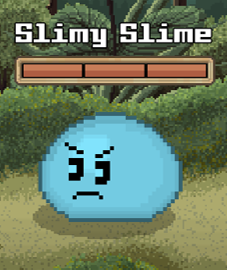
\includegraphics[width=5cm]{Images/Monster.png}
	\vspace{0.5cm}
	\caption{Quái vật}
\end{figure}
\hspace*{0.5cm} Quái vật chính là đối thủ của người chơi, và sẽ là đối trọng của người chơi trong chiến đấu. Quái vật thường sẽ đứng phía bên phải của khu vực chiến đấu. Trên đầu quái vật gồm tên quái vật và một thanh trạng thái của các bộ phận chí mạng, lưu ý rằng nó không thể hiện điểm máu của các bộ phận mà nó chỉ biểu thị trạng thái tồn tại của các bộ phận của quái vật.\\
\hspace*{0.5cm} Mỗi loại quái vật có thể có các ngoại hình khác nhau. Ngoại hình quái vật mà người chơi nhìn thấy bằng mắt có thể là gợi ý giúp người chơi khai thác schema nói chung, bảng \textbf{Knowledge} có hiệu quả thông qua các gợi ý về màu sắc, hoa văn, kỹ năng, các đặc điểm bên ngoài lẫn bên trong,... Ngoài ra, người chơi cũng có thể xâu chuỗi các thông tin trong schema và ngoại hình bên ngoài để có thể tìm được các mã định danh của quái vật và bộ phận quái vật đúng một cách hiệu quả.\\

\subsubsection{Thông số, trang bị và kho đồ}
\begin{figure}[H]
	\centering
	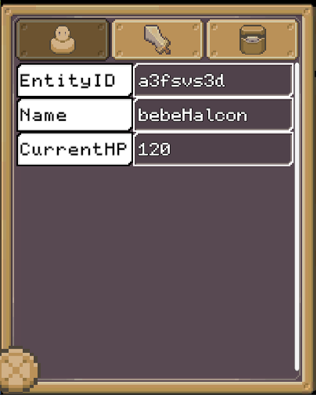
\includegraphics[width=10cm]{Images/Inventory.png}
	\vspace{0.5cm}
	\caption{Thông số, trang bị và kho đồ}
\end{figure}
\hspace*{0.5cm} Đây là khu vực chứa các thông tin của nhân vật chính, tức là người chơi. Giao diện gồm 3 tabs
\begin{itemize}
	\item User Stats: Tab này là nơi chứa thông số của người chơi hiện tại. Bao gồm entityID, tên người chơi, máu hiện tại, trạng thái hiệu ứng hiện tại, cùng các thông tin khác
	\item Equipment: Chứa thông tin các món trang bị được trang bị trong các slots trang bị của người chơi. Chủ yếu chứa thông tin của các món trang bị bao gồm hình ảnh, loại trang bị và tên trang bị, khi người chơi di chuột vào icon của trang bị, toàn bộ thông tin của trang bị sẽ được hiện ra.
	\item Inventory: Chứa thông tin các món vật phẩm trong kho đồ, tương tự với trang bị, các row trong tab này chủ yếu chứa thông tin của các vật phẩm bao gồm hình ảnh, loại vật phẩm và tên của nó, khi người chơi di chuột vào icon, toàn bộ thông tin của vật phẩm sẽ được hiện ra. Các vật phẩm tiêu hao (bình hồi máu, bình giải hiệu ứng) sẽ được ưu tiên hiện lên trên đầu.
\end{itemize}
\hspace*{0.5cm} Thông tin của người chơi luôn được cập nhật kịp thời để người chơi có thể dễ dàng nắm bắt tình trạng nhân vật người chơi đang điều khiển.
\subsubsection{Ô nhập lệnh và kết quả truy vấn}
\begin{figure}[H]
	\centering
	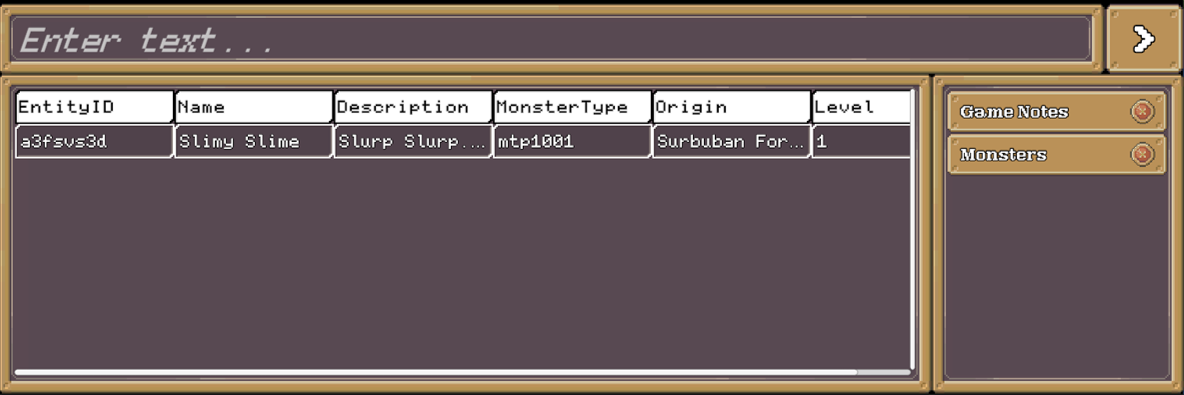
\includegraphics[width=10cm]{Images/CommandBox.png}
	\vspace{0.5cm}
	\caption{Ô nhập lệnh và kết quả truy vấn}
\end{figure}
\hspace*{0.5cm} Đây là nơi diễn ra các hoạt động nhập câu truy vấn và nhận về kết quả dưới dạng bảng. Bảng kết quả gồm hàng đầu chứa header của bảng, các hàng tiếp theo chứa nội dung các hàng tương ứng trong bảng. Người chơi có thể di chuột vào ô để xem toàn bộ nội dung của bảng cũng như click vào ô để sao chép nội dung của ô đó vào clipboard. Người chơi cũng có thể nhập các câu lệnh truy vấn insert vào các bảng đặc biệt để ra lệnh người chơi tấn công vào mục tiêu được chỉ định.\\
\hspace*{0.5cm} Phía bên phải sẽ là một vùng chứa các tab đến các bảng đã được query. Người chơi có thể chuyển qua lại giữa các tab, cũng như đóng các tab không cần dùng đến. Khi người chơi select một bảng không có trong tab, thì tab mới sẽ được tạo ra với nội dung là kết quả trả về của bảng vừa truy vấn.
\hspace*{0.5cm} Bên cạnh đó là một tab "Game Notes". Nó hoạt động như một cuốn sổ note, nó giúp người chơi ghi chú lại những dữ kiện trong quá trình khai thác schema, thay vì phải mở một chương trình text editor bên ngoài, thì chỉ cần sử dụng tab này thì có thể ghi lại những ghi chú mà người chơi mong muốn.
\subsubsection{Phong cảnh màn chơi và khu vực hiện tại}
\begin{figure}[H]
	\centering
	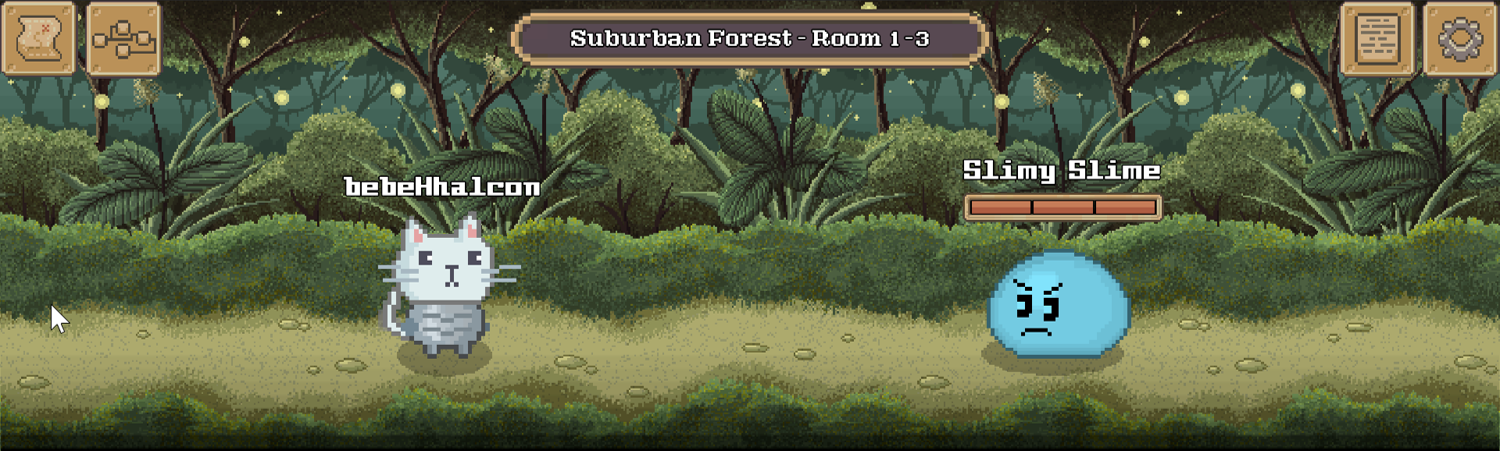
\includegraphics[width=10cm]{Images/CurrentRoom.png}
	\vspace{0.5cm}
	\caption{Quang cảnh môi trường của khu vực chơi hiện tại}
\end{figure}
\hspace*{0.5cm} Đây là khu vực chơi của trò chơi, nơi môi trường được thể hiện trên màn hình.\\
\hspace*{0.5cm} Phía trên là phần giao diện phía trên. Vùng ở giữa chứa tên màn chơi và khu vực hiện tại của người chơi. Đi kèm với các nút theo thứ tự từ trái sang phải sẽ là: 
\begin{enumerate}
	\item Nút Map: Mở bản đồ của màn chơi.
	\item Nút Schema: Mở Schema Diagram của game.
	\item Nút Documentation: Mở Documentation của SQLite.
	\item Nút Settings: Mở hộp thoại Settings.
\end{enumerate}